Este anexo se organiza en tres bloques. El primero (C.1--C.5) reúne el material de consulta: el
mapa de señales completo entre los conectores FMC de la ZCU102 y las placas LINCE Comunicación
Serial, CDHS y AOCS, la tabla de frecuencias soportadas por el NCO del transceptor serie junto con
su error medido, y el recuento del código desarrollado a lo largo del trabajo. El segundo
(C.6--C.8) recoge el detalle de implementación que el Capítulo~3 deja fuera para no interrumpir el
hilo: la descripción RTL de los bloques auxiliares del transceptor, la aplicación de testing del
driver serie y el procedimiento completo del ejemplo con el que se validó el flujo de desarrollo.
El tercero (C.9--C.10) contiene los volcados completos del terminal de las pruebas de validación
hardware del Capítulo~4.

\section{Mapa de señales LINCE Comunicación Serial} \label{anxC:mapa_serial}

La tabla~\ref{tab:mapa_lince_serial} recoge el mapeado de los 14 drivers RS485/RS422 de la placa
LINCE Comunicación Serial con el conector FMC HPC0 (P2) de la ZCU102. Cada driver expone las
señales TX, RX, SLO y DE (esta última ausente en los drivers 7 y 11, que solo disponen de
control de dirección hardware).

{\footnotesize
\begin{longtable}{llllll}
    \hline
    \textbf{Driver} & \textbf{Señal} & \textbf{Red Interna} & \textbf{Red (FMC HPC0)} & \textbf{Pin FMC (P2)} & \textbf{Pin Zynq} \\
    \hline
    \endfirsthead
    \hline
    \textbf{Driver} & \textbf{Señal} & \textbf{Red Interna} & \textbf{Red (FMC HPC0)} & \textbf{Pin FMC (P2)} & \textbf{Pin Zynq} \\
    \hline
    \endhead
    \hline
    \endfoot
    \hline
    \caption{Mapa de señales entre la placa LINCE Comunicación Serial y el conector FMC HPC0 (P2) de la ZCU102.}
    \label{tab:mapa_lince_serial}
    \endlastfoot
    Driver0 & TX  & TX0   & FMC\_HPC0\_LA32\_N      & H38 & T11  \\
    Driver0 & RX  & RX0   & FMC\_HPC0\_LA26\_N      & D27 & K15  \\
    Driver0 & SLO & SLO0  & FMC\_HPC0\_LA27\_N      & C27 & L10  \\
    Driver0 & DE  & DE0   & FMC\_HPC0\_LA33\_N      & G37 & V11  \\
    Driver1 & TX  & TX1   & FMC\_HPC0\_LA33\_P      & G36 & V12  \\
    Driver1 & RX  & RX1   & FMC\_HPC0\_LA30\_N      & H35 & U6   \\
    Driver1 & SLO & SLO1  & FMC\_HPC0\_LA32\_P      & H37 & U11  \\
    Driver1 & DE  & DE1   & FMC\_HPC0\_LA27\_P      & C26 & M10  \\
    Driver2 & TX  & TX2   & FMC\_HPC0\_LA30\_P      & H34 & V6   \\
    Driver2 & RX  & RX2   & FMC\_HPC0\_LA26\_P      & D26 & L15  \\
    Driver2 & SLO & SLO2  & FMC\_HPC0\_LA31\_N      & G34 & V7   \\
    Driver2 & DE  & DE2   & FMC\_HPC0\_LA31\_P      & G33 & V8   \\
    Driver3 & TX  & TX3   & FMC\_HPC0\_LA29\_N      & G31 & U8   \\
    Driver3 & RX  & RX3   & FMC\_HPC0\_LA29\_P      & G30 & U9   \\
    Driver3 & SLO & SLO3  & FMC\_HPC0\_LA28\_N      & H32 & T6   \\
    Driver3 & DE  & DE3   & FMC\_HPC0\_LA28\_P      & H31 & T7   \\
    Driver4 & TX  & TX4   & FMC\_HPC0\_LA14\_P      & C18 & AC7  \\
    Driver4 & RX  & RX4   & FMC\_HPC0\_LA13\_N      & D18 & AC8  \\
    Driver4 & SLO & SLO4  & FMC\_HPC0\_LA22\_P      & G24 & M15  \\
    Driver4 & DE  & DE4   & FMC\_HPC0\_LA19\_N      & H23 & K13  \\
    Driver5 & TX  & TX5   & FMC\_HPC0\_LA20\_N      & G22 & M13  \\
    Driver5 & RX  & RX5   & FMC\_HPC0\_LA15\_N      & H20 & Y9   \\
    Driver5 & SLO & SLO5  & FMC\_HPC0\_LA19\_P      & H22 & L13  \\
    Driver5 & DE  & DE5   & FMC\_HPC0\_LA20\_P      & G21 & N13  \\
    Driver6 & TX  & TX6   & FMC\_HPC0\_LA15\_P      & H19 & Y10  \\
    Driver6 & RX  & RX6   & FMC\_HPC0\_LA13\_P      & D17 & AB8  \\
    Driver6 & SLO & SLO6  & FMC\_HPC0\_LA16\_N      & G19 & AA12 \\
    Driver6 & DE  & DE6   & FMC\_HPC0\_LA16\_P      & G18 & Y12  \\
    Driver7 & TX  & TX7   & FMC\_HPC0\_LA06\_P      & C10 & AC2  \\
    Driver7 & RX  & RX7   & FMC\_HPC0\_LA01\_CC\_N  & D9  & AC4  \\
    Driver7 & SLO & SLO7  & FMC\_HPC0\_LA01\_CC\_P  & D8  & AB4  \\
    Driver8 & TX  & TX8   & FMC\_HPC0\_LA05\_P      & D11 & AB3  \\
    Driver8 & RX  & RX8   & FMC\_HPC0\_LA05\_N      & D12 & AC3  \\
    Driver8 & SLO & SLO8  & FMC\_HPC0\_LA06\_N      & C11 & AC1  \\
    Driver8 & DE  & DE8   & FMC\_HPC0\_LA10\_P      & C14 & W5   \\
    Driver9 & TX  & TX9   & FMC\_HPC0\_LA02\_P      & H7  & V2   \\
    Driver9 & RX  & RX9   & FMC\_HPC0\_LA00\_CC\_N  & G7  & Y3   \\
    Driver9 & SLO & SLO9  & FMC\_HPC0\_LA00\_CC\_P  & G6  & Y4   \\
    Driver9 & DE  & DE9   & FMC\_HPC0\_LA02\_N      & H8  & V1   \\
    Driver10 & TX  & TX10  & FMC\_HPC0\_LA09\_P     & D14 & W2   \\
    Driver10 & RX  & RX10  & FMC\_HPC0\_LA03\_N     & G10 & Y1   \\
    Driver10 & SLO & SLO10 & FMC\_HPC0\_LA03\_P     & G9  & Y2   \\
    Driver10 & DE  & DE10  & FMC\_HPC0\_LA04\_P     & H10 & AA2  \\
    Driver11 & TX  & TX11  & FMC\_HPC0\_LA08\_N     & G13 & V3   \\
    Driver11 & RX  & RX11  & FMC\_HPC0\_LA08\_P     & G12 & V4   \\
    Driver11 & SLO & SLO11 & FMC\_HPC0\_LA04\_N     & H11 & AA1  \\
    Driver12 & TX  & TX12  & FMC\_HPC0\_LA10\_N     & C15 & W4   \\
    Driver12 & RX  & RX12  & FMC\_HPC0\_LA07\_N     & H14 & U4   \\
    Driver12 & SLO & SLO12 & FMC\_HPC0\_LA07\_P     & H13 & U5   \\
    Driver12 & DE  & DE12  & FMC\_HPC0\_LA09\_N     & D15 & W1   \\
    Driver13 & TX  & TX13  & FMC\_HPC0\_LA11\_N     & H17 & AB5  \\
    Driver13 & RX  & RX13  & FMC\_HPC0\_LA11\_P     & H16 & AB6  \\
    Driver13 & SLO & SLO13 & FMC\_HPC0\_LA12\_P     & G15 & W7   \\
    Driver13 & DE  & DE13  & FMC\_HPC0\_LA12\_N     & G16 & W6   \\
\end{longtable}
}

\section{Mapa de señales CDHS} \label{anxC:mapa_cdhs}

La tabla~\ref{tab:mapa_cdhs} recoge el mapeado de los cuatro subsistemas de la placa CDHS (SPI del
ADC, CAN nominal y redundante, los tres canales serie y las cuatro líneas de PWM) con el conector
FMC HPC0 de la ZCU102.

\begin{table}[H]
    \centering
    \small
    \begin{tabular}{llllll}
        \hline
        \textbf{Subsistema} & \textbf{Señal} & \textbf{Red (FMC HPC0)} & \textbf{Pin FMC} & \textbf{Pin Zynq} \\
        \hline
        SPI (ADC) & SDO & FMC\_HPC0\_LA02\_N & H8 & V1 \\
        SPI (ADC) & SDI & FMC\_HPC0\_LA00\_CC\_N & G7 & Y3 \\
        SPI (ADC) & SCLK & FMC\_HPC0\_LA02\_P & H7 & V2 \\
        SPI (ADC) & CS\_N & FMC\_HPC0\_LA00\_CC\_P & G6 & Y4 \\
        CAN (Nominal) & TX\_N & FMC\_HPC0\_LA21\_P & H25 & P12 \\
        CAN (Nominal) & RX\_N & FMC\_HPC0\_LA22\_P & G24 & M15 \\
        CAN (Redundante) & TX\_R & FMC\_HPC0\_LA21\_N & H26 & N12 \\
        CAN (Redundante) & RX\_R & FMC\_HPC0\_LA22\_N & G25 & M14 \\
        RS1 (Serial 1) & TX & FMC\_HPC0\_LA15\_P & H19 & Y10 \\
        RS1 (Serial 1) & RX & FMC\_HPC0\_LA11\_N & H17 & AB5 \\
        RS1 (Serial 1) & DE & FMC\_HPC0\_LA16\_P & G18 & Y12 \\
        RS2 (Serial 2) & TX & FMC\_HPC0\_LA12\_N & G16 & W6 \\
        RS2 (Serial 2) & RX & FMC\_HPC0\_LA12\_P & G15 & W7 \\
        RS2 (Serial 2) & DE & FMC\_HPC0\_LA11\_P & H16 & AB6 \\
        RS3 (Serial 3) & TX & FMC\_HPC0\_LA07\_N & H14 & U4 \\
        RS3 (Serial 3) & RX & FMC\_HPC0\_LA07\_P & H13 & U5 \\
        RS3 (Serial 3) & DE & FMC\_HPC0\_LA08\_N & G13 & V3 \\
        PWM (Heaters) & IN1 & FMC\_HPC0\_LA04\_N & H11 & AA1 \\
        PWM (Heaters) & IN2 & FMC\_HPC0\_LA04\_P & H10 & AA2 \\
        PWM (Heaters) & IN3 & FMC\_HPC0\_LA03\_P & G9 & Y2 \\
        PWM (Heaters) & IN4 & FMC\_HPC0\_LA03\_N & G10 & Y1 \\
        \hline
    \end{tabular}
    \caption{Mapa de señales entre la placa CDHS y el conector FMC HPC0 de la ZCU102.}
    \label{tab:mapa_cdhs}
\end{table}

\section{Mapa de señales AOCS} \label{anxC:mapa_aocs}

El mapa de la tabla~\ref{tab:mapa_aocs} corresponde a la revisión V2 de la placa, la versión
cerrada del esquemático (sección~\ref{sec:diseno_aocs}). Respecto a la revisión fabricada, cada canal serie consume
cuatro señales del FMC en lugar de tres, porque las líneas DE y RE dejan de estar
cortocircuitadas, y el conector J4 alberga dos canales (RS41 y RS42).

{\small
\begin{longtable}{lllll}
    \caption{Mapa de señales entre la revisión V2 de la placa AOCS y el conector FMC HPC0 de la
    ZCU102.} \label{tab:mapa_aocs} \\
    \hline
    \textbf{Subsistema} & \textbf{Señal} & \textbf{Red (FMC HPC0)} & \textbf{Pin FMC} & \textbf{Pin Zynq} \\
    \hline
    \endfirsthead
    \hline
    \textbf{Subsistema} & \textbf{Señal} & \textbf{Red (FMC HPC0)} & \textbf{Pin FMC} & \textbf{Pin Zynq} \\
    \hline
    \endhead
    \hline
    \endfoot
    RS1 (Serial J1) & TX & FMC\_HPC0\_LA19\_P & H22 & L13 \\
    RS1 (Serial J1) & RX & FMC\_HPC0\_LA17\_CC\_N & D21 & N11 \\
    RS1 (Serial J1) & DE & FMC\_HPC0\_LA18\_CC\_P & C22 & N9 \\
    RS1 (Serial J1) & RE & FMC\_HPC0\_LA20\_P & G21 & N13 \\
    MOT-PWM (J2) & PWM\_X\_1 & FMC\_HPC0\_LA17\_CC\_P & D20 & P11 \\
    MOT-PWM (J2) & PWM\_X\_2 & FMC\_HPC0\_LA15\_N & H20 & Y9 \\
    MOT-PWM (J2) & PWM\_Y\_1 & FMC\_HPC0\_LA16\_N & G19 & AA12 \\
    MOT-PWM (J2) & PWM\_Y\_2 & FMC\_HPC0\_LA15\_P & H19 & Y10 \\
    MOT-PWM (J2) & PWM\_Z\_1 & FMC\_HPC0\_LA16\_P & G18 & Y12 \\
    MOT-PWM (J2) & PWM\_Z\_2 & FMC\_HPC0\_LA13\_N & D18 & AC8 \\
    RS3 (Serial J3) & TX & FMC\_HPC0\_LA11\_N & H17 & AB5 \\
    RS3 (Serial J3) & RX & FMC\_HPC0\_LA11\_P & H16 & AB6 \\
    RS3 (Serial J3) & DE & FMC\_HPC0\_LA14\_P & C18 & AC7 \\
    RS3 (Serial J3) & RE & FMC\_HPC0\_LA13\_P & D17 & AB8 \\
    RS41 (Serial J4) & TX & FMC\_HPC0\_LA12\_N & G16 & W6 \\
    RS41 (Serial J4) & RX & FMC\_HPC0\_LA09\_N & D15 & W1 \\
    RS41 (Serial J4) & DE & FMC\_HPC0\_LA10\_N & C15 & W4 \\
    RS41 (Serial J4) & RE & FMC\_HPC0\_LA12\_P & G15 & W7 \\
    RS42 (Serial J4) & TX & FMC\_HPC0\_LA07\_N & H14 & U4 \\
    RS42 (Serial J4) & RX & FMC\_HPC0\_LA07\_P & H13 & U5 \\
    RS42 (Serial J4) & DE & FMC\_HPC0\_LA09\_P & D14 & W2 \\
    RS42 (Serial J4) & RE & FMC\_HPC0\_LA08\_N & G13 & V3 \\
    RS5 (Serial J5) & TX & FMC\_HPC0\_LA05\_N & D12 & AC3 \\
    RS5 (Serial J5) & RX & FMC\_HPC0\_LA05\_P & D11 & AB3 \\
    RS5 (Serial J5) & DE & FMC\_HPC0\_LA08\_P & G12 & V4 \\
    RS5 (Serial J5) & RE & FMC\_HPC0\_LA06\_N & C11 & AC1 \\
    SPW1 (J6) & DIN\_P & FMC\_HPC0\_LA02\_P & H7 & V2 \\
    SPW1 (J6) & DIN\_N & FMC\_HPC0\_LA02\_N & H8 & V1 \\
    SPW1 (J6) & SIN\_P & FMC\_HPC0\_LA04\_P & H10 & AA2 \\
    SPW1 (J6) & SIN\_N & FMC\_HPC0\_LA04\_N & H11 & AA1 \\
    SPW1 (J6) & SOUT\_P & FMC\_HPC0\_LA01\_CC\_P & D8 & AB4 \\
    SPW1 (J6) & SOUT\_N & FMC\_HPC0\_LA01\_CC\_N & D9 & AC4 \\
    SPW1 (J6) & DOUT\_P & FMC\_HPC0\_LA00\_CC\_P & G6 & Y4 \\
    SPW1 (J6) & DOUT\_N & FMC\_HPC0\_LA00\_CC\_N & G7 & Y3 \\
    SPW2 (J7) & DIN\_P & FMC\_HPC0\_LA24\_P & H28 & L12 \\
    SPW2 (J7) & DIN\_N & FMC\_HPC0\_LA24\_N & H29 & K12 \\
    SPW2 (J7) & SIN\_P & FMC\_HPC0\_LA21\_P & H25 & P12 \\
    SPW2 (J7) & SIN\_N & FMC\_HPC0\_LA21\_N & H26 & N12 \\
    SPW2 (J7) & SOUT\_P & FMC\_HPC0\_LA28\_P & H31 & T7 \\
    SPW2 (J7) & SOUT\_N & FMC\_HPC0\_LA28\_N & H32 & T6 \\
    SPW2 (J7) & DOUT\_P & FMC\_HPC0\_LA30\_P & H34 & V6 \\
    SPW2 (J7) & DOUT\_N & FMC\_HPC0\_LA30\_N & H35 & U6 \\
    RS8 (Serial J8) & TX & FMC\_HPC0\_LA22\_P & G24 & M15 \\
    RS8 (Serial J8) & RX & FMC\_HPC0\_LA20\_N & G22 & M13 \\
    RS8 (Serial J8) & DE & FMC\_HPC0\_LA19\_N & H23 & K13 \\
    RS8 (Serial J8) & RE & FMC\_HPC0\_LA23\_P & D23 & L16 \\
    \hline
\end{longtable}
}

\section{Tabla de frecuencias del NCO} \label{anxC:nco}

La tabla del NCO del transceptor serie contiene \textbf{54 entradas}, de 50 a 4\,000\,000 de
baudios. La tabla~\ref{tab:nco} recoge las \textbf{29 que ejercita el \textit{testbench}}
\texttt{tb\_NCO.vhd}, que son las del rango de uso previsto (de 9\,600 a 3,6864~Mbaudios): para cada
una, los dos valores de incremento que la función de síntesis calcula (el nominal y el de doble
frecuencia) y la frecuencia medida en simulación, con su error en ppm respecto a la nominal. Las
entradas por debajo de 9\,600~baudios quedan fuera del uso previsto y la de 4~Mbaudios exige un
tiempo de simulación desproporcionado, de modo que ninguna de ellas se barre.

\begin{table}[H]
    \centering
    \small
    \begin{tabular}{rrrrrr}
        \hline
        \textbf{Baud} & \textbf{Half} & \textbf{INC\_ROM} & \textbf{INC\_HALF\_ROM} & \textbf{Medido (Hz)} & \textbf{Error (ppm)} \\
        \hline
        9\,600   & 0 & 412\,316    & 824\,633    & 9\,600,002    & 0,2 \\
        14\,400  & 0 & 618\,475    & 1\,236\,950   & 14\,399,988   & $-$0,8 \\
        19\,200  & 0 & 824\,633    & 1\,649\,267   & 19\,200,012   & 0,6 \\
        28\,800  & 0 & 1\,236\,950   & 2\,473\,901   & 28\,799,977   & $-$0,8 \\
        31\,250  & 0 & 1\,342\,177   & 2\,684\,354   & 31\,250,000   & 0,0 \\
        38\,400  & 0 & 1\,649\,267   & 3\,298\,534   & 38\,400,025   & 0,6 \\
        56\,000  & 0 & 2\,405\,181   & 4\,810\,363   & 55\,999,978   & $-$0,4 \\
        57\,600  & 0 & 2\,473\,901   & 4\,947\,802   & 57\,600,037   & 0,6 \\
        74\,400  & 0 & 3\,195\,455   & 6\,390\,911   & 74\,400,057   & 0,8 \\
        115\,200 & 0 & 4\,947\,802   & 9\,895\,604   & 115\,200,074  & 0,6 \\
        128\,000 & 0 & 5\,497\,558   & 10\,995\,116  & 128\,000,000  & 0,0 \\
        153\,600 & 0 & 6\,597\,069   & 13\,194\,139  & 153\,600,393  & 2,6 \\
        230\,400 & 0 & 9\,895\,604   & 19\,791\,209  & 230\,398,820  & $-$5,1 \\
        256\,000 & 0 & 10\,995\,116  & 21\,990\,232  & 256\,000,000  & 0,0 \\
        312\,500 & 0 & 13\,421\,772  & 26\,843\,545  & 312\,500,000  & 0,0 \\
        460\,800 & 0 & 19\,791\,209  & 39\,582\,418  & 460\,808,258  & 17,9 \\
        500\,000 & 0 & 21\,474\,836  & 42\,949\,672  & 500\,000,000  & 0,0 \\
        576\,000 & 0 & 24\,739\,011  & 49\,478\,023  & 576\,003,686  & 6,4 \\
        614\,400 & 0 & 26\,388\,279  & 52\,776\,558  & 614\,401,573  & 2,6 \\
        750\,000 & 0 & 32\,212\,254  & 64\,424\,509  & 749\,990,625  & $-$12,5 \\
        921\,600 & 0 & 39\,582\,418  & 79\,164\,837  & 921\,616,515  & 17,9 \\
        1\,000\,000 & 0 & 42\,949\,672 & 85\,899\,345  & 1\,000\,000,000 & 0,0 \\
        1\,152\,000 & 0 & 49\,478\,023 & 98\,956\,046  & 1\,152\,007,373 & 6,4 \\
        1\,500\,000 & 0 & 64\,424\,509 & 128\,849\,018 & 1\,499\,925,004 & $-$50,0 \\
        1\,843\,200 & 0 & 79\,164\,837 & 158\,329\,674 & 1\,843\,148,097 & $-$28,2 \\
        2\,000\,000 & 0 & 85\,899\,345 & 171\,798\,691 & 2\,000\,000,000 & 0,0 \\
        2\,500\,000 & 0 & 107\,374\,182 & 214\,748\,364 & 2\,500\,000,000 & 0,0 \\
        3\,000\,000 & 0 & 128\,849\,018 & 257\,698\,037 & 3\,000\,300,030 & 100,0 \\
        3\,686\,400 & 0 & 158\,329\,674 & 316\,659\,348 & 3\,685\,956,506 & $-$120,3 \\
        \hline
    \end{tabular}
    \caption{Velocidades del NCO verificadas en simulación.}
    \label{tab:nco}
\end{table}

\section{Volumen y distribución del código desarrollado} \label{anxC:loc}

Se recoge aquí el recuento de líneas de código de autoría propia escritas en el trabajo, desglosado
por lenguaje y por función. El criterio de recuento es restrictivo: se excluye todo el código
generado automáticamente por las herramientas (los IP de AMD, los ficheros que Vivado produce al
empaquetar un IP o al sintetizar un diseño de bloques), el código de terceros incorporado al
proyecto (el sistema de compilación \texttt{waf} de RTEMS, el árbol de dispositivos de Xilinx) y las
copias de un mismo fichero replicadas entre las distintas variantes del proyecto, de las que se
contabiliza únicamente la versión final.

\begin{table}[H]
    \centering
    \begin{tabular}{llrr}
        \hline
        \textbf{Lenguaje} & \textbf{Función} & \textbf{Líneas} & \textbf{Peso} \\
        \hline
        TCL   & Automatización del flujo de Vivado          & 5\,338  & 26,4\,\% \\
        VHDL  & RTL sintetizable (transceptor, puente)      & 4\,710  & 23,3\,\% \\
        VHDL  & \textit{Testbenches} de simulación          & 4\,551  & 22,5\,\% \\
        C     & Driver RTEMS y aplicaciones de prueba       & 2\,617  & 13,0\,\% \\
        Python& Utilidades de instrumentación y GUI         & 1\,525  & 7,6\,\% \\
        Bash  & Compilación y despliegue de imágenes        & 1\,231  & 6,1\,\% \\
        XDC   & \textit{Constraints} de la FPGA             & 216    & 1,1\,\% \\
        \hline
        \multicolumn{2}{l}{\textbf{Total}} & \textbf{20\,188} & \textbf{100\,\%} \\
        \hline
    \end{tabular}
    \caption{Distribución de las líneas de código desarrolladas en el trabajo.}
    \label{tab:loc}
\end{table}

La distribución es en sí misma un resultado, y admite dos lecturas que respaldan los principios
metodológicos enunciados en la sección de metodología.

La primera es que el \textbf{código de verificación pesa prácticamente lo mismo que el código que
verifica}: 4\,551 líneas de \textit{testbench} frente a 4\,710 de VHDL sintetizable, una relación de
0,97:1. Por cada línea de hardware descrita se escribió casi una línea destinada exclusivamente a
comprobarla en simulación, lo que cuantifica la política de no integrar ningún bloque sin
verificación previa aislada.

La segunda es que la \textbf{automatización es la mayor partida del trabajo}: TCL, Bash y Python
suman 8\,094 líneas, el 40,1\,\% del total, por encima de cualquier otra categoría y muy por encima
del código de aplicación. Es la traducción cuantitativa de una decisión deliberada, la de invertir por
adelantado en herramientas que hicieran el flujo reproducible y barato de iterar, cuyo retorno se
manifestó en las campañas de depuración, donde regenerar el diseño completo desde cero pasó a ser
un comando en lugar de una tarde de trabajo manual.

\section{Descripción RTL del registro de desplazamiento y la FIFO} \label{anxC:rtl_fifo}

Este apartado detalla los dos bloques auxiliares situados entre el receptor y el PS, cuyo
comportamiento se resume en la sección~\ref{sec:normalizacion_fifo} del capítulo de desarrollo.

\subsection{Registro de desplazamiento}

El registro de desplazamiento convierte a paralelo los bits que va entregando el receptor. Sus
entradas son el bit muestreado (\texttt{D}), un pulso de habilitación por bit recibido
(\texttt{Enable}, conectado al \texttt{Valid\_out} del receptor) y las dos señales de configuración
que determinan el formato de la palabra (\texttt{data\_bits} y \texttt{bit\_order}); su salida
\texttt{Q} es la palabra de 9~bits. El registro solo evoluciona en los ciclos en que
\texttt{Enable} está activo, de modo que la FSM del receptor controla exactamente qué muestras
entran en la palabra.

Está diseñado para poder almacenar datos tanto si la configuración es LSB-\textit{first} como
MSB-\textit{first}, de modo que una vez recibido el mensaje la palabra en la salida siempre es la
correcta independientemente del modo configurado. Para ello dispone de dos caminos de
desplazamiento combinacionales, seleccionados por \texttt{bit\_order}: en LSB \textit{first} el
bit entrante se inserta en la posición más significativa de la palabra activa y el contenido se
desplaza hacia la derecha; en MSB \textit{first} se inserta en la posición cero y el contenido se
desplaza hacia la izquierda. Cada camino tiene a su vez cinco variantes, una por anchura de
palabra, que fijan dónde se inserta el bit y rellenan a cero las posiciones no utilizadas.

El efecto de esta \textbf{normalización} es que, completada la trama, el primer bit de datos
recibido ocupa siempre \texttt{Q(0)} y la palabra está alineada al LSB con independencia de la
configuración. Los dos consumidores de la salida, la FIFO y el cálculo de paridad esperada del
receptor, pueden así ignorar por completo el orden de bits configurado, y el software del PS
recibe la palabra en el mismo formato en los cinco anchos y en los dos órdenes posibles.

\subsection{FIFO}

La FIFO es un bloque IP con 9 bits de datos (para poder almacenar mensajes de 9 bits) y
512 de profundidad, que permite almacenar temporalmente varios mensajes y habilitarlos
para su lectura posterior por el PS. Está configurada en modo \textit{first word fall through},
de modo que la palabra más antigua está disponible en la salida sin necesidad de una lectura
previa, y su reset síncrono se deriva del reset global del transceptor. La escritura la ordena
directamente el pulso \texttt{Store\_out} del receptor, que solo se emite cuando la trama ha
superado las comprobaciones de paridad y bit de parada.

La habilitación de lectura se construye como la conjunción de FIFO no vacía y la señal
\texttt{Data\_read} procedente del PS. Esta última se toma \textbf{a nivel}: en la versión inicial
se empleaba el flanco detectado de \texttt{Data\_read}, lo que resulta adecuado cuando el PS lee
byte a byte, pero deja de serlo con el transporte por DMA descrito en la
sección~\ref{sec:transporte_desarrollo}, donde \texttt{Data\_read} lo conduce la señal
\textit{tready} del canal AXI-Stream. La latencia del detector de flanco, de dos etapas de
registro, hacía que el receptor de DMA capturase varias veces la misma palabra de la FIFO. Con
la lectura a nivel, la FIFO avanza exactamente en el ciclo en que el consumidor acepta el dato.

\section{Aplicación de testing del driver serie en RTEMS} \label{anxC:testing_driver}

Este apartado detalla la aplicación de pruebas con la que se ejercitó el driver serie sobre la
ZCU102, resumida en la sección~\ref{sec:testing_driver} del capítulo de desarrollo. Está repartida
en tres ficheros: \texttt{init.c}, con la configuración estática del sistema; el driver
(\texttt{transceiver.c} y \texttt{transceiver.h}); y \texttt{main.c}, con la aplicación propiamente
dicha.

\subsection{Configuración del sistema --- \texttt{init.c}}

\texttt{init.c} no contiene lógica de aplicación. Define el entorno de ejecución mediante macros
que \texttt{<rtems/confdefs.h>} convierte en estructuras de datos internas del núcleo.

\begin{lstlisting}[style=terminal, caption={Configuración estática de RTEMS en init.c}]
CONFIGURE_APPLICATION_NEEDS_CLOCK_DRIVER    // rtems_task_wake_after()
CONFIGURE_APPLICATION_NEEDS_CONSOLE_DRIVER // stdin/stdout (printf, fgets)
CONFIGURE_MICROSECONDS_PER_TICK 10000       // Tick = 10 ms (100 Hz)
CONFIGURE_UNLIMITED_OBJECTS                 // Sin limite de tareas/semaforos
CONFIGURE_UNIFIED_WORK_AREAS               // Un unico pool de memoria
CONFIGURE_INIT_TASK_STACK_SIZE (64 KB)    // Stack grande para Init
\end{lstlisting}

\subsection{Aplicación --- \texttt{main.c}}

La aplicación tiene tres secciones claramente separadas.

\textbf{Callback de recepción \texttt{on\_rx\_data()}.} Se registra en el driver y se invoca desde
la tarea \textit{worker} cuando llegan datos. Implementa un ensamblador de líneas por canal: por
cada byte recibido acumula hasta encontrar un carácter de fin de línea (\verb|\n| o \verb|\r|),
momento en el que imprime la línea completa con el formato \texttt{[RX UART 02]: mensaje}. Hay un
\texttt{AppLineBuffer} de 1024 bytes por cada uno de los 14 canales, declarado estáticamente en el
array \texttt{rx\_lines[MAX\_TRANSCEIVERS]}. Esto evita mezclar caracteres de UART distintas en la
misma línea de consola.

\textbf{Tarea de consola de transmisión \texttt{Tx\_Console\_Task()}.} Es una tarea de RTEMS
independiente, de prioridad 100, que bloquea en \texttt{fgets(stdin)} esperando comandos del
usuario por la consola USB. El protocolo de comandos es el siguiente.

\begin{lstlisting}[caption={Protocolo de comandos de la aplicación de testing}]
<ID> <MENSAJE>     -> Envia MENSAJE por la UART numero ID
ALL <MENSAJE>      -> Envia MENSAJE por TODAS las UARTs
<ID> SLO ON        -> Reconfigura UART ID con Slew Rate limitado
<ID> SLO OFF       -> Reconfigura UART ID con Slew Rate normal
ALL SLO ON/OFF     -> Aplica configuracion SLO a todas las UARTs
\end{lstlisting}

Los comandos SLO reejecutan \texttt{Transceiver\_Init()} con una configuración distinta, lo que
permite reconfigurar el hardware en caliente sin reiniciar el sistema.

\textbf{Función \texttt{Init()}.} RTEMS la llama al arrancar en lugar de \texttt{main()}. La
secuencia de inicialización es:

\begin{enumerate}
    \item \texttt{mmu\_map\_pl\_axi\_early()}: mapea en la MMU la región de la PL para acceso
    \textit{bare-metal}.
    \item \texttt{Transceiver\_Global\_INIT()}: descubre el hardware e instala la ISR maestra.
    \item Bucle de inicialización: para cada UART se invoca \texttt{Transceiver\_Init()}, se
    registra su \textit{callback} de recepción y se envía el mensaje de disponibilidad del canal.
    \item Creación y lanzamiento de \texttt{Tx\_Console\_Task}.
    \item \texttt{rtems\_task\_delete(RTEMS\_SELF)}: la tarea Init se elimina a sí misma; el
    núcleo queda con las tareas \textit{worker} y la tarea de consola.
\end{enumerate}

\section{Flujo de desarrollo de extremo a extremo: ejemplo de la puerta AND} \label{anxC:flujo_and}

Este apartado recoge el procedimiento completo del ejemplo de validación descrito en el
apartado~\ref{sec:flujo_extremo_a_extremo}: la puerta AND descrita en VHDL y sintetizada en la PL,
la imagen de arranque que la lleva a la placa y la traza que confirma su funcionamiento. El
proyecto completo, con el diseño y el código de las dos mitades, está en
\texttt{tfm/00\_docs/AND\_example} dentro del repositorio del proyecto~\cite{repo_tfm}.

\subsection{Descripción VHDL y \textit{Block Design}}

El proyecto de Vivado, llamado \texttt{and\_gate\_ps\_p}, parte de la descripción de la puerta:

\begin{lstlisting}[language=VHDL, caption={AND\_GATE.vhd}]
library IEEE;
use IEEE.STD_LOGIC_1164.ALL;

entity AND_GATE is
    Port ( A_B_IN : in  STD_LOGIC_VECTOR (1 downto 0);
           Z_OUT  : out STD_LOGIC);
end AND_GATE;

architecture Behavioral of AND_GATE is
begin
    Z_OUT <= A_B_IN(1) and A_B_IN(0);
end Behavioral;
\end{lstlisting}

Sobre un \textit{Block Design} nuevo se añadió el bloque Zynq UltraScale+ MPSoC IP, configurado con
la \textit{Block Automation} de Vivado, el fichero VHDL anterior y dos AXI GPIO IP para comunicar
el PS con la PL. Las conexiones restantes se resolvieron con \textit{Automate Connection}. El
resultado es la figura~\ref{fig:block_design_and}, y en ella se aprecia la estructura que se repite
en todos los diseños del trabajo: el bloque del PS, los periféricos de la PL y el interconector AXI
que los une, con el bloque VHDL propio colgando de uno de los dos AXI GPIO.

\begin{figure}[htbp]
    \centering
    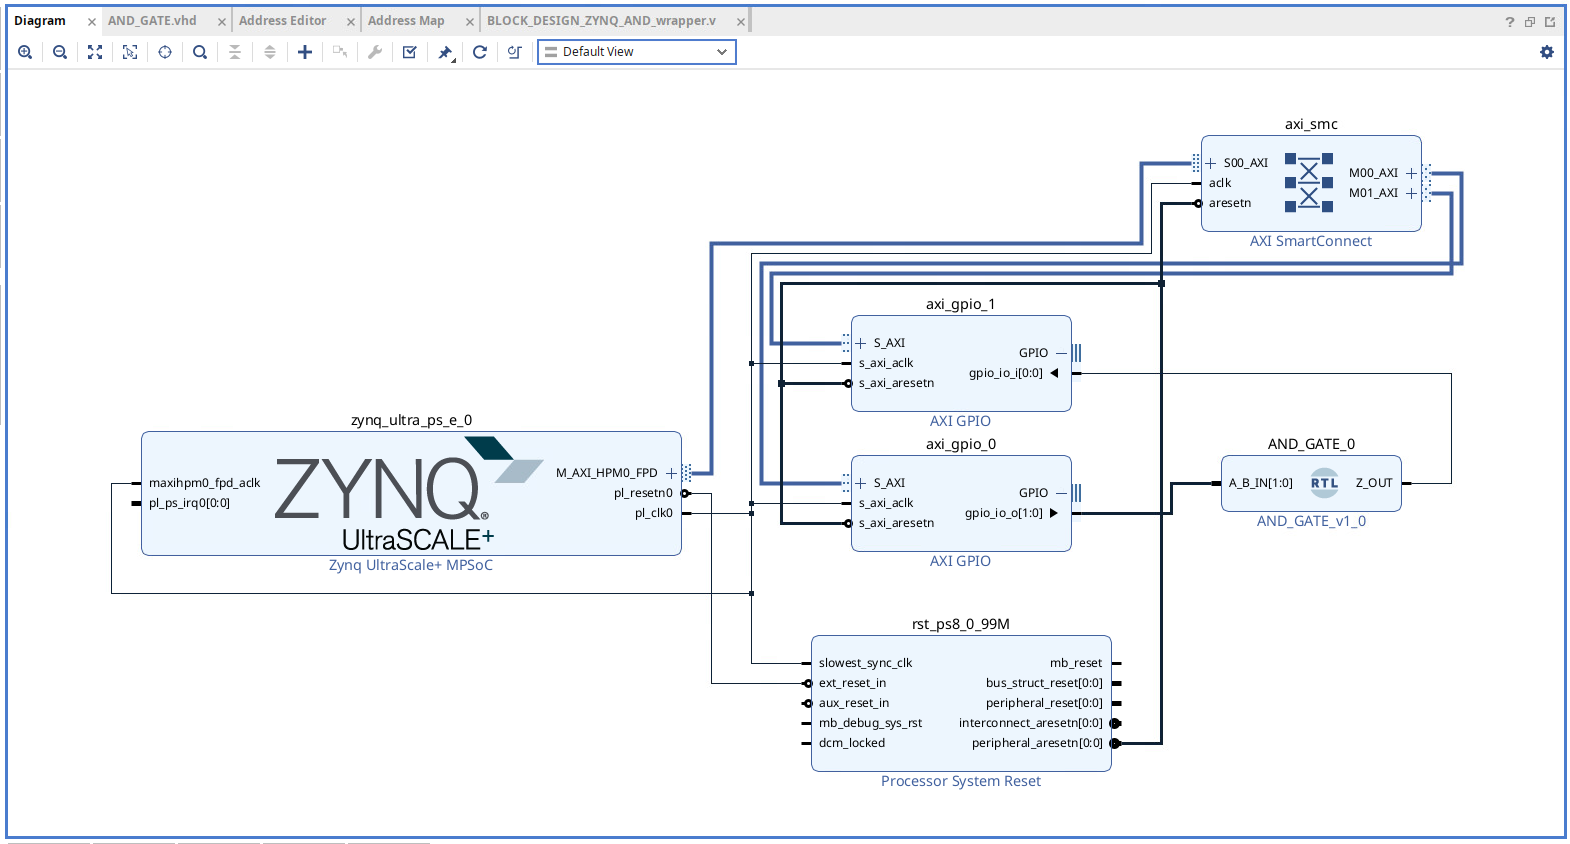
\includegraphics[width=\textwidth]{IMG/Desarrollo/block_design_and.png}
    \caption{\textit{Block Design} del ejemplo de la puerta AND.}
    \label{fig:block_design_and}
\end{figure}

Después se creó un \textit{Wrapper} del \textit{Block Design} para que Vivado pudiera sintetizarlo.
La pestaña \textit{Address Editor} lista las direcciones base con las que el PS accede a los
registros de cada periférico de la PL. Por último se generó el \textit{BitStream} y se exportó el
hardware como .xsa.

\subsection{Generación de la imagen de arranque en Vitis}

Este paso empaqueta el hardware generado en Vivado, junto con el software de arranque, en el único
binario que el MPSoC ejecuta desde la tarjeta SD:

\begin{enumerate}
    \item Se creó un componente de tipo \textit{Platform} en Vitis, tomando como base el .xsa
    exportado desde Vivado, y se compiló.
    \item Sobre esa plataforma se creó una aplicación a partir del ejemplo \textit{Zynq MP FSBL},
    el cargador de arranque de primera etapa (\textit{First Stage Boot Loader}), que es el primer
    programa que ejecuta el PS y el que carga el resto de componentes de la imagen. Al compilarla
    se obtiene el \texttt{zynqmp\_fsbl\_proyect.elf}.
    \item Se lanzó el generador de imágenes de Vitis (\textit{Create Zynq UltraScale+ Boot Image})
    y se añadieron los componentes en el orden de la figura~\ref{fig:vitis_boot_image}, ya que el
    orden dentro del fichero BIF (\textit{Boot Image Format}) determina la secuencia de arranque.
\end{enumerate}

El modo y el orden de los componentes dentro del BIF son la parte del procedimiento que la
documentación de AMD no reúne en un solo sitio, y un error en cualquiera de los dos impide el
arranque sin dar un mensaje útil. De ahí el detalle de la lista siguiente:

\begin{itemize}
    \item \texttt{zynqmp\_fsbl\_proyect.elf}, en modo \textit{bootloader}, destino a53-0 y nivel
    de excepción EL3. Se encuentra en la carpeta \texttt{build} de la aplicación anterior.
    \item \texttt{pmufw.elf}, en modo \textit{pmufw\_image} y destino a53-0. Es el firmware de la
    unidad de gestión de potencia y se descargó del repositorio de firmware precompilado de
    AMD para la ZCU102\footnote{\url{https://github.com/Xilinx/soc-prebuilt-firmware/tree/xilinx_v2025.1/zcu102-zynqmp}}.
    \item \texttt{BLOCK\_DESIGN\_ZYNQ\_AND\_wrapper.bit}, en modo \textit{datafile} y con la PL
    como dispositivo de destino. Es el \textit{bitstream} generado por Vivado.
    \item \texttt{bl31.elf}, en modo \textit{datafile}, destino a53-0 y nivel de excepción EL3. Es
    el firmware de ARM Trusted Firmware y se descarga del mismo sitio que el PMUFW.
    \item \texttt{u-boot.elf}, en modo \textit{datafile}, destino a53-0 y nivel de excepción EL2.
    U-Boot es un gestor de arranque de segunda etapa. Se ejecuta después del FSBL, inicializa
    los periféricos necesarios (tarjeta SD, red, consola serie) y carga en memoria la imagen
    del sistema operativo (en este caso \texttt{rtems.img}), a la que cede el control.
    Ofrece además una consola interactiva desde la que se puede inspeccionar la memoria o
    elegir manualmente qué imagen arrancar, lo que resultó útil durante la depuración.
    \item \texttt{system.dtb}, en modo \textit{datafile}, destino a53-0 y dirección de carga
    \texttt{0x100000}. Este árbol de dispositivos en binario (DTB) es el que permite a BL31 saber
    dónde está enlazado el BL33 (U-Boot) y arrancarlo.
\end{itemize}

\begin{figure}[htbp]
    \centering
    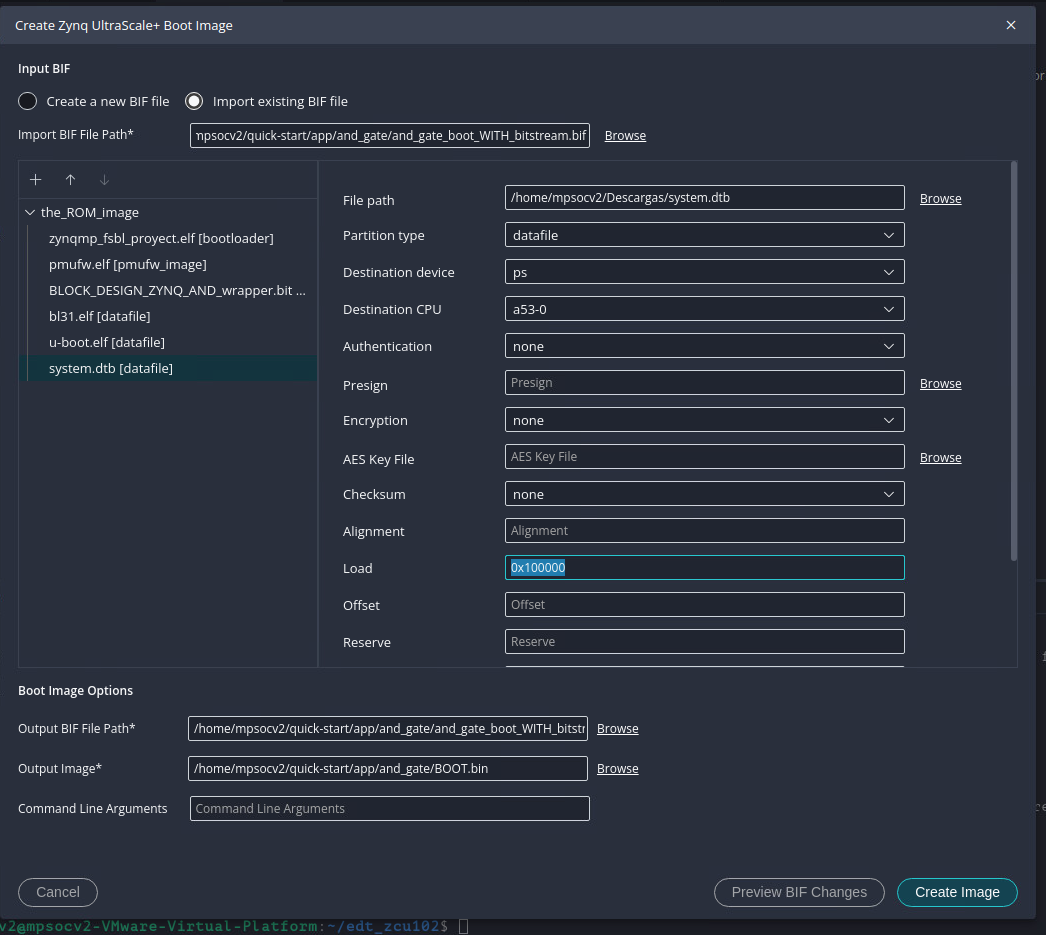
\includegraphics[width=\textwidth]{IMG/Desarrollo/vitis_boot_image.png}
    \caption{Generador de imágenes de arranque de Vitis.}
    \label{fig:vitis_boot_image}
\end{figure}

\subsection{Aplicación de RTEMS y arranque desde la tarjeta SD}

La aplicación se reparte en dos fuentes. \texttt{and\_demo.c} contiene la tarea \texttt{Init}:
escribe la pareja de entradas \texttt{(A,B)} en el registro de datos del \texttt{axi\_gpio\_0}
(mapeado en \texttt{0xA0000000}), espera un instante a que la lógica de la PL se estabilice, lee la
salida \texttt{Z} del \texttt{axi\_gpio\_1} (\texttt{0xA0010000}) e imprime cada resultado por la
consola serie. \texttt{mmu\_pl\_map.c} declara como memoria de periférico el rango
\texttt{0xA0000000}--\texttt{0xA01FFFFF}, donde Vivado ha situado los AXI GPIO; el mapeado se
realiza nada más arrancar \texttt{Init}, porque RTEMS desconoce a priori las direcciones de la PL.
La compilación necesita además un \texttt{wscript}.

Los dos ficheros, \texttt{BOOT.BIN} y \texttt{rtems.img}, se copian en la partición FAT de una
tarjeta SD, que se inserta en el zócalo \texttt{J100} de la placa~\cite{xilinx2023ug1182}. El
\texttt{BOOT.BIN} es el que el MPSoC ejecuta nada más alimentarse: inicializa el PS, carga el
\textit{bitstream} en la PL y encadena el resto de etapas hasta U-Boot, que a su vez carga el
\texttt{rtems.img} en memoria y le cede el control. Si el ensayo solo ejercita la PL, el
\texttt{BOOT.BIN} basta por sí solo, ya que lleva dentro el \textit{bitstream}.

Antes de encender la placa hay que colocar el selector de modo de arranque en la posición de
tarjeta SD. Es el conmutador DIP \texttt{SW6}, la referencia 44 del plano de componentes de la
ZCU102~\cite{xilinx2023ug1182}, cuyas posiciones recoge la tabla~\ref{tab:sw6}. Conviene tenerlo
presente porque la configuración de fábrica es \texttt{QSPI32}: sin cambiar el conmutador, la
placa no arranca desde la tarjeta aunque los ficheros estén correctamente copiados.

\begin{table}[H]
    \centering
    \begin{tabular}{lcc}
        \hline
        \textbf{Modo de arranque} & \textbf{\texttt{PS\_MODE[3:0]}} & \textbf{SW6 [4:1]} \\
        \hline
        JTAG                      & 0000 & ON, ON, ON, ON \\
        QSPI32 (por defecto)      & 0010 & ON, ON, OFF, ON \\
        \textbf{Tarjeta SD}       & 1110 & \textbf{OFF, OFF, OFF, ON} \\
        \hline
    \end{tabular}
    \caption{Posiciones del selector de modo de arranque SW6 de la ZCU102
    \cite{xilinx2023ug1182}.}
    \label{tab:sw6}
\end{table}

\subsection{Barrido de la tabla de verdad}

Con la tarjeta insertada y el conmutador en su sitio, el barrido completo sale por la consola
serie:

\begin{lstlisting}[caption={Salida de terminal --- barrido de la puerta AND}]
## Transferring control to RTEMS (at address 000100000) ...
Barrido AND via PL
A=0, B=0, Z=0 (raw=0x00000000)
A=0, B=1, Z=0 (raw=0x00000000)
A=1, B=0, Z=0 (raw=0x00000000)
A=1, B=1, Z=1 (raw=0x00000001)

[ RTEMS shutdown ]
\end{lstlisting}

La primera línea la emite U-Boot al ceder el control a la imagen de RTEMS. Las cuatro siguientes
son las escritas por \texttt{and\_demo.c}, con la salida \texttt{Z} a uno únicamente cuando ambas
entradas valen uno. La salida se conserva en
\texttt{tfm/\allowbreak 00\_docs/\allowbreak logs\_terminal/\allowbreak and\_gate\_output.txt}.

\section{Volcados completos de terminal de las pruebas serie RS422/RS485} \label{anxC:volcados_serie}

Este apartado recoge la salida íntegra del terminal de las dos sesiones de prueba de
comunicaciones serie RS422/RS485 descritas en las secciones~\ref{sec:cdhs_rs} y
\ref{sec:validacion_aocs} del capítulo de validación hardware.

\subsection{Placa CDHS (3 transceptores)} \label{anxC:volcado_cdhs}

La sesión recoge el descubrimiento dinámico de los tres transceptores instanciados en el
\textit{bitstream} y los intercambios de \textit{loopback} entre UART~0, UART~1 y UART~2.

\begin{lstlisting}[style=terminal, caption={Salida completa del terminal --- prueba RS422/RS485 con la placa CDHS (3 transceptores)}]
MMU_MAP: return from mmu_map_pl_axi_early()
[TRANSCEIVER DEBUG] Detectados: 3 | Base: 0xA0000000 | INT: 0xA0003000
[TRANSCEIVER DEBUG]   - Transceptor 0: 0xA0000000
[TRANSCEIVER DEBUG]   - Transceptor 1: 0xA0001000
[TRANSCEIVER DEBUG]   - Transceptor 2: 0xA0002000

=== ARRANQUE SISTEMA ZCU102 (5 UARTs) ===
UART 00 [OK] Base: 0xA0000000
UART 01 [OK] Base: 0xA0001000
UART 02 [OK] Base: 0xA0002000
[RX UART 00]: UART 2 Lista.

=======================================================
 CONSOLA DE CONTROL MULTI-TRANSCEPTOR
-------------------------------------------------------
 Formato: <ID> <MENSAJE> | <ID> SLO ON | <ID> SLO OFF
 Ejemplos:
   '0 Hola'      -> Envia 'Hola' por UART 0
   'ALL Reset'   -> Envia 'Reset' por TODAS las UARTs
   '2 SLO ON'    -> Activa el modo Slow Rate en UART 2
   'ALL SLO OFF' -> Desactiva el modo Slow en TODAS
=======================================================

CMD>
---- Sent utf8 encoded message: "0 hola" ----
0 hola
Tx -> UART 0: OK
CMD> [RX UART 02]: hola
---- Sent utf8 encoded message: "2 hola" ----
2 hola
Tx -> UART 2: OK
CMD> [RX UART 00]: hola
---- Sent utf8 encoded message: "0 hola" ----
0 hola
Tx -> UART 0: OK
CMD> [RX UART 02]: hola
---- Sent utf8 encoded message: "2 hola" ----
2 hola
Tx -> UART 2: OK
CMD> [RX UART 00]: hola
---- Sent utf8 encoded message: "0 hola" ----
0 hola
Tx -> UART 0: OK
CMD> [RX UART 02]: ?hola
---- Sent utf8 encoded message: "2 hola" ----
2 hola
Tx -> UART 2: OK
CMD> [RX UART 00]: ?hola
---- Sent utf8 encoded message: "0 hola" ----
0 hola
Tx -> UART 0: OK
CMD> [RX UART 02]: ?hola
---- Sent utf8 encoded message: "2 hola" ----
2 hola
Tx -> UART 2: OK
CMD> [RX UART 00]: ?hola
---- Sent utf8 encoded message: "0 hola" ----
0 hola
Tx -> UART 0: OK
CMD> [RX UART 02]: hola
---- Sent utf8 encoded message: "2 hola" ----
2 hola
Tx -> UART 2: OK
CMD> [RX UART 00]: hola
---- Sent utf8 encoded message: "0 HOLA MUNDO" ----
0 HOLA MUNDO
Tx -> UART 0: OK
CMD> [RX UART 02]: HOLA MUNDO
---- Sent utf8 encoded message: "1 HOLA MUNDO" ----
1 HOLA MUNDO
Tx -> UART 1: OK
CMD>
---- Sent utf8 encoded message: "2 HOLA MUNDO" ----
2 HOLA MUNDO
Tx -> UART 2: OK
CMD> [RX UART 00]: HOLA MUNDO
\end{lstlisting}

\subsection{Placa AOCS (5 transceptores)} \label{anxC:volcado_aocs}

La sesión recoge el descubrimiento dinámico de los cinco transceptores instanciados en el
\textit{bitstream} y los cuatro pares de \textit{loopback} ejercitados entre UART~0 y el
resto de canales.

\begin{lstlisting}[style=terminal, caption={Salida completa del terminal --- prueba RS422/RS485 con la placa AOCS (5 transceptores)}]
MMU_MAP: return from mmu_map_pl_axi_early()
[TRANSCEIVER DEBUG] Detectados: 5 | Base: 0xA0000000 | INT: 0xA0005000
[TRANSCEIVER DEBUG]   - Transceptor 0: 0xA0000000
[TRANSCEIVER DEBUG]   - Transceptor 1: 0xA0001000
[TRANSCEIVER DEBUG]   - Transceptor 2: 0xA0002000
[TRANSCEIVER DEBUG]   - Transceptor 3: 0xA0003000
[TRANSCEIVER DEBUG]   - Transceptor 4: 0xA0004000

=== ARRANQUE SISTEMA ZCU102 (5 UARTs) ===
UART 00 [OK] Base: 0xA0000000
UART 01 [OK] Base: 0xA0001000
UART 02 [OK] Base: 0xA0002000
UART 03 [OK] Base: 0xA0003000
UART 04 [OK] Base: 0xA0004000
[RX UART 00]: UART 4 Lista.

=======================================================
 CONSOLA DE CONTROL MULTI-TRANSCEPTOR
-------------------------------------------------------
 Formato: <ID> <MENSAJE> | <ID> SLO ON | <ID> SLO OFF
 Ejemplos:
   '0 Hola'      -> Envia 'Hola' por UART 0
   'ALL Reset'   -> Envia 'Reset' por TODAS las UARTs
   '2 SLO ON'    -> Activa el modo Slow Rate en UART 2
   'ALL SLO OFF' -> Desactiva el modo Slow en TODAS
=======================================================

CMD>
---- Sent utf8 encoded message: "0 HOLA" ----
0 HOLA
Tx -> UART 0: OK
CMD> [RX UART 04]: HOLA
---- Sent utf8 encoded message: "4 HOLA" ----
4 HOLA
Tx -> UART 4: OK
CMD> [RX UART 00]: HOLA
---- Sent utf8 encoded message: "0 HOLA" ----
0 HOLA
Tx -> UART 0: OK
CMD> [RX UART 03]: HOLA
---- Sent utf8 encoded message: "3 HOLA" ----
3 HOLA
Tx -> UART 3: OK
CMD> [RX UART 00]: HOLA
---- Sent utf8 encoded message: "0 HOLA" ----
0 HOLA
Tx -> UART 0: OK
CMD> [RX UART 02]: HOLA
---- Sent utf8 encoded message: "2 HOLA" ----
2 HOLA
Tx -> UART 2: OK
CMD> [RX UART 00]: HOLA
---- Sent utf8 encoded message: "0 HOLA" ----
0 HOLA
Tx -> UART 0: OK
CMD> [RX UART 01]: HOLA
---- Sent utf8 encoded message: "1 HOLA" ----
1 HOLA
Tx -> UART 1: OK
CMD> [RX UART 00]: HOLA
\end{lstlisting}

\section{Volcado completo del barrido del ADC} \label{anxC:volcado_adc}

Este apartado recoge la salida íntegra del terminal del barrido de tensión aplicado al canal
CH2 del ADC ADS7950 de la placa CDHS, descrito en la sección~\ref{sec:validacion_cdhs} del
capítulo de validación hardware. Se aprecian los dos tramos de subida y bajada de la rampa
aplicada a CH2, los dos escalones intermedios en los que la fuente se dejó fija y la
estabilidad de los otros tres canales durante todo el ensayo.

\begin{lstlisting}[style=terminal, caption={Salida completa del terminal --- barrido de tensión sobre CH2 del ADS7950 (placa CDHS)}]
ADS7950: CH0= 244  CH1=  43  CH2=   0  CH3=  19
ADS7950: CH0= 243  CH1=  43  CH2=   0  CH3=  19
ADS7950: CH0= 244  CH1=  43  CH2=   0  CH3=  19
ADS7950: CH0= 245  CH1=  43  CH2=   0  CH3=  19
ADS7950: CH0= 244  CH1=  43  CH2=   0  CH3=  19
ADS7950: CH0= 245  CH1=  44  CH2=   0  CH3=  19
ADS7950: CH0= 244  CH1=  43  CH2=1577  CH3=  19
ADS7950: CH0= 245  CH1=  43  CH2=1577  CH3=  19
ADS7950: CH0= 244  CH1=  43  CH2=1579  CH3=  19
ADS7950: CH0= 245  CH1=  43  CH2=1582  CH3=  19
ADS7950: CH0= 245  CH1=  43  CH2=1580  CH3=  20
ADS7950: CH0= 245  CH1=  43  CH2=1827  CH3=  19
ADS7950: CH0= 245  CH1=  43  CH2=2156  CH3=  20
ADS7950: CH0= 245  CH1=  44  CH2=2501  CH3=  20
ADS7950: CH0= 245  CH1=  43  CH2=2814  CH3=  20
ADS7950: CH0= 246  CH1=  43  CH2=2934  CH3=  21
ADS7950: CH0= 245  CH1=  43  CH2=3419  CH3=  21
ADS7950: CH0= 245  CH1=  43  CH2=3565  CH3=  21
ADS7950: CH0= 245  CH1=  43  CH2=3535  CH3=  22
ADS7950: CH0= 245  CH1=  43  CH2=3536  CH3=  22
ADS7950: CH0= 246  CH1=  43  CH2=3069  CH3=  22
ADS7950: CH0= 246  CH1=  43  CH2=2770  CH3=  22
ADS7950: CH0= 246  CH1=  43  CH2=2436  CH3=  22
ADS7950: CH0= 247  CH1=  43  CH2=1896  CH3=  22
ADS7950: CH0= 246  CH1=  43  CH2=1509  CH3=  22
ADS7950: CH0= 246  CH1=  43  CH2=1276  CH3=  22
ADS7950: CH0= 247  CH1=  43  CH2= 928  CH3=  22
ADS7950: CH0= 246  CH1=  43  CH2= 433  CH3=  22
ADS7950: CH0= 247  CH1=  43  CH2= 400  CH3=  22
ADS7950: CH0= 247  CH1=  43  CH2= 583  CH3=  22
ADS7950: CH0= 246  CH1=  43  CH2=1238  CH3=  22
ADS7950: CH0= 247  CH1=  43  CH2=1808  CH3=  23
ADS7950: CH0= 247  CH1=  43  CH2=1827  CH3=  23
ADS7950: CH0= 247  CH1=  43  CH2=1826  CH3=  23
ADS7950: CH0= 248  CH1=  43  CH2= 647  CH3=  23
ADS7950: CH0= 248  CH1=  44  CH2= 245  CH3=  23
ADS7950: CH0= 248  CH1=  43  CH2= 189  CH3=  23
ADS7950: CH0= 248  CH1=  43  CH2= 166  CH3=  22
ADS7950: CH0= 247  CH1=  43  CH2= 148  CH3=  23
ADS7950: CH0= 248  CH1=  43  CH2= 130  CH3=  22
ADS7950: CH0= 248  CH1=  43  CH2= 116  CH3=  22
ADS7950: CH0= 248  CH1=  43  CH2= 102  CH3=  22
ADS7950: CH0= 248  CH1=  43  CH2=1823  CH3=  23
ADS7950: CH0= 247  CH1=  43  CH2=1821  CH3=  23
ADS7950: CH0= 248  CH1=  43  CH2=1820  CH3=  23
ADS7950: CH0= 248  CH1=  43  CH2=1825  CH3=  23
ADS7950: CH0= 248  CH1=  43  CH2=1826  CH3=  23
ADS7950: CH0= 250  CH1=  43  CH2=1826  CH3=  23
ADS7950: CH0= 249  CH1=  43  CH2=1826  CH3=  23
ADS7950: CH0= 249  CH1=  44  CH2=1827  CH3=  23
ADS7950: CH0= 249  CH1=  43  CH2=1825  CH3=  23
ADS7950: CH0= 249  CH1=  43  CH2=1826  CH3=  24
ADS7950: CH0= 248  CH1=  43  CH2=1820  CH3=  24
ADS7950: CH0= 249  CH1=  43  CH2= 390  CH3=  23
ADS7950: CH0= 249  CH1=  43  CH2= 230  CH3=  23
ADS7950: CH0= 250  CH1=  43  CH2= 189  CH3=  23
\end{lstlisting}
